\documentclass{beamer}

\usepackage[spanish,activeacute,es-tabla]{babel}
\usepackage[utf8]{inputenc} % mac utf8
%\usepackage{beamerthemesplit}


\usepackage{graphicx}
\DeclareGraphicsExtensions{.png,.pdf,.jpg}


\usefonttheme{professionalfonts} % fuentes de LaTeX 
\usetheme{Boadilla}	% tema escogido en este ejemplo 

\setbeamertemplate{caption}[numbered]


\newtheorem{Teorema}{Teorema} 
\newtheorem{Ejemplo}{Ejemplo} 
\newtheorem{Definicion}{Definici\’on} 
\newtheorem{Corolario}{Corolario} 
\newtheorem{Prueba}{Prueba}

\newtheorem{teorema} [Teorema] {Teorema}
\newtheorem{ejemplo} [Ejemplo] {Ejemplo}
\newtheorem{definicion} [Definicion]{Definición} 
\newtheorem{ejercicio} [Corolario]{Ejercicio} 
\newtheorem{lema} [theorem] {Lema}

\setbeamertemplate{theorems}[numbered] 





\title[]{Tema 1. Codificación y sus usos}
\author[José A Montenegro (jmmontes@uma.es)]{José A. Montenegro}
\institute{Dpto. Lenguajes y Ciencias de la Computación\\
ETSI Informática. Universidad de Málaga\\
jmmontes@uma.es
%\href{https://twitter.com//monteDocencia}{
%
\includegraphics[height=0.03\textheight]{twitter.jpg}}
}
\date{\today}

%###########################################################################
% FootLine
%###########################################################################

\setbeamertemplate{footline} {%
\leavevmode%
  \hbox{\begin{beamercolorbox}[wd=.5\paperwidth,ht=2.5ex,dp=1.125ex,leftskip=.3cm plus1fill,rightskip=.3cm]{author in head/foot}%
    \usebeamerfont{author in head/foot}\insertshortauthor 
  \end{beamercolorbox}%
  
  \begin{beamercolorbox}[wd=.5\paperwidth,ht=2.5ex,dp=1.125ex,leftskip=.3cm,rightskip=.3cm plus1fil]{title in head/foot}%
    Teoría de la Información y Codificación \hfill    \insertpagenumber /\insertdocumentendpage
  \end{beamercolorbox}}%
  \vskip0pt%
}%

%###########################################################################
% Document
%###########################################################################

\begin{document}

%\setbeamertemplate{headline}[title slide]
%\setbeamertemplate{footline}[title slide]


%###########################################################################
% Tíitulo
%###########################################################################
\begin{frame}

\includegraphics[height=0.15\textheight]{logoUma.jpg} \hspace*{3.5cm}

\includegraphics[height=0.17\textheight]{logoInf.jpg}   \hspace*{3.5cm}

\includegraphics[height=0.17\textheight]{logoLcc.jpg}  

\titlepage


\setbeamertemplate{footline}[body]
\setbeamertemplate{headline}[body]
\end{frame}

%###########################################################################
% Contenidos
%###########################################################################
\small
\section[Resumen]{}
\frame{\tableofcontents}

%%%%%%%%%%%%%%%%%%%%%%%%%%%%%%%%
%%%%%%%%%%%%%%%%%%%%%%%%%%%%%%%%
%SECCION %%%%%%%%%%%%%%%%%%%%%%%%%%%%%%%
%%%%%%%%%%%%%%%%%%%%%%%%%%%%%%%%
%%%%%%%%%%%%%%%%%%%%%% 

%%%%%%%%%%%%%%%%%%%%%%%%%%%%%%%%
%%%%%%%%%%%%%%%%%%%%%%%%%%%%%%%%
%\begin{frame}  \small \begin{ejercicio} \end{ejercicio} \pause \textit{\underline{Solución}}:\\ \end{frame} 
%%%%%%%%%%%%%%%%%%%%%%%%%%%%%%%%
%%%%%%%%%%%%%%%%%%%%%%%%%%%%%%%%
%EJERCICIO %%%%%%%%%%%%%%%%%%%%%%%%%%%%%%%
%%%%%%%%%%%%%%%%%%%%%%%%%%%%%%%%

%%%%%%%%%%%%%%%%%%%%%%%%%%%%%%%%
%\begin{frame}  \small  
%\begin{itemize} \item  \item \item \item 
%\end{itemize} \end{frame} 

%%%%%%%%%%%%%%%%%%%%%%%%%%%%%%%%
%\begin{frame}  \small  
%\end{frame} 


%%%%%%%%%%%%%%%%%%%%%% 

\section{Mensajes}

\subsection{Definición Informal}

\begin{frame}  \frametitle{Mensajes}    \small
  La primera tarea que debemos realizar es establecer el modelo matemático de un mensaje. 
  
\begin{ejemplo}
Muchos mensajes están escritos en un lenguaje natural, como es el caso del Español.\\

Estos mensajes contienen símbolos y los símbolos forman palabras, los cuales constituyen frases.\\

\vspace{0,5cm}
Los mensajes pueden ser enviados de una persona a otra utilizando varios medios: una nota manuscrita, un correo electrónico, mensaje, etc. 
 
\end{ejemplo}
\end{frame}

\begin{frame}

\small

\begin{ejemplo}
Dispositivos como los escáners y cámaras digitales producen mensajes utilizando impulsos electrónicos. Estos mensajes pueden ser enviados de un dispositivo a otro mediante cables, o mediante ondas de radio.
\end{ejemplo}

Las definiciones formales basadas en estos ejemplos serán establecidas más adelante. 


\begin{itemize}
\item Por ahora, estableceremos que un \textbf{mensaje} es una secuencia de símbolos, teniendo en cuenta que el orden de los símbolos es muy importante. 

\item  La \textbf{principal función} de un mensaje es transportar información de un ente a otro. 

\item Los elementos de la comunicación deben estar de acuerdo en el mismo conjunto de símbolos, denominado \textbf{Alfabeto}.

\end{itemize}


\end{frame}



\begin{frame}   
    
\begin{ejemplo}
Denotamos por $\mathbb{A}$ el alfabeto que tiene 28 símbolos, las letras \textit{\{A,B,C,D,E,F,G,H,I,J,K,L,M,N,Ñ,O,P,Q,R,S,T,U,V,W,X,Y,Z\}} y un espacio, el cual es denotado por $\sqcup$ (28 ó 0).

\vspace{0,25cm}
Utilizaremos el alfabeto $\mathbb{A}$ para representar los mensajes escritos en Español.

\vspace{0,25cm} 
Ignoramos elementos del idioma, distinción entre mayúsculas y minúscula, así como marcas de puntuación. 

\end{ejemplo}

\begin{center}
En un lugar de la Mancha ... 
\end{center}

es reducido al siguiente mensaje utilizando el alfabeto  $\mathbb{A}$.

\begin{center}
$\mathtt{EN\sqcup UN\sqcup LUGAR\sqcup DE\sqcup LA\sqcup MANCHA}$ 
\end{center}
  
 \end{frame}
 
 \begin{frame}   
 
 \begin{ejemplo}
El alfabeto $\mathbb{B}$ tiene dos símbolos, 0 y 1, determinados dígitos binarios o bits.\\
\vspace{0,25cm}
Bits 0 y 1 son implementados electrónicamente como estados APAGADO y ENCENCIDO.\\ 
\vspace{0,25cm}

En la práctica, los bits son combinados en grupos, como palabras de 32 bits.\\
\vspace{1cm}
Cualquier mensaje transmitido electrónicamente  es esencialmente una secuencia de bits.
\end{ejemplo}
  
\end{frame}


%%%%%%%%%%%%%%%%%%%%%%%%%%%%%%% SECTION

\section{Codificación}
\subsection{Aproximación al problema}

\begin{frame}   \frametitle{Codificación} 

\begin{itemize}
\item \textbf{Codificar} es definido como una regla que permite una sustitución de un mensaje por otro mensaje.
\item Los mensajes no tienen que compartir los mismos alfabetos.
\end{itemize}
    

\begin{ejemplo}
Una simple regla para codificar un mensaje en el alfabeto $\mathbb{A}$  utilizando el mismo alfabeto es: \textit{escribir cada palabra al revés}. Por lo que el mensaje:


\begin{center}
$\mathtt{NOS}\sqcup\mathtt{VEMOS}\sqcup\mathtt{PRONTO}$   sería   $\mathtt{SON}\sqcup\mathtt{SOMEV}\sqcup\mathtt{OTNORP}$ 
\end{center}

\end{ejemplo}

\end{frame}

%%%%%%%%%%%%%%%%%%%%%%%%%%%%%%%%%

\begin{frame} 

\begin{ejemplo}
Una regla para codificar mensajes en $\mathbb{A}$  utilizando el alfabeto $\mathbb{B}$ es: \textit{reemplazar las vocales por ceros y las consonantes por unos}. Por lo que el mensaje:

\begin{center}
$\mathtt{NOS}\sqcup\mathtt{VEMOS}\sqcup\mathtt{PRONTO}$   sería  $10110101110110$
\end{center}
   
    \end{ejemplo}
    
Hasta ahora ejemplos mostrados son artificiales tienen un valor limitado.\\
\vspace{0,5cm}

Debemos mirar los propósitos de la codificación para acercarnos a la realidad. 

\end{frame}

%%%%%%%%%%%%%%%%%%%%%%%%%%%%%%%%

\subsection{Razones codificación mensajes}
\begin{frame}
Hay tres razones principales para codificar un mensaje:

\small
\begin{description}

\item[Económicas:] Situaciones es necesario utilizar un alfabeto menor que los lenguajes naturales. O es deseable el mensaje más pequeño, esto ha dado lugar al desarrollo de técnicas  para la \textit{Compresión de datos}. 

\item[Fiabilidad:] El proceso de transmisión no está libre de ``ruido'' que proporciona alteraciones en los mensajes. Necesario desarrollar \textit{Corrección de los Errores}.


\item[Seguridad:] Usualmente es necesaria la confidencialidad de los mensajes. Históricamente, desarrollada en las comunicaciones diplomáticas y militares, pero hoy en día juegan en todas las transacciones económicas.  Este área de codificación es conocida como \textit{Criptografía}. 
\end{description}


\end{frame}


%%%%%%%%%%%%%%%%%EJERCICIO

\begin{frame} 

\small

\begin{itemize}
\item Otros usos como \textit{Algoritmos de Predicción} en el caso de dispositivos de tamaño reducido.

\end{itemize}


\begin{ejercicio}
 Los siguientes mensajes son versiones codificadas del Español. Determine las reglas de codificación utilizadas y encuentre el mensaje original.

\begin{center}
20     22     5     19     21    5
\end{center}

\begin{center}
10100	10110	00101	10011		10101		00101
\end{center}	

\end{ejercicio}
%%%%%%%%%%%%%%%%%EJERCICIO

\end{frame}

\section{Definiciones Formales}\label{sec:defba}

\subsection{Alfabetos, Símbolos, Mensajes y Cadena}

\begin{frame} \frametitle{Definiciones Formales}


\begin{definicion} [Alfabeto y Símbolos]
Un Alfabeto es un conjunto finito S. Los miembros de S son denominados símbolos.
\end{definicion}


\begin{definicion} [Mensaje, cadena y palabra]
Un mensaje en el alfabeto S es una secuencia finita de miembros de S:

\begin{center} $x_{1}x_{2} \ldots x_{n} (x_{i} \in S, 1 \leq i \leq n).$\end{center}
Un mensaje es una cadena de miembros de S, o una palabra en S, donde n es la longitud del mensaje, cadena o palabra.
\end{definicion}

\end{frame}

%%%%%%%%%%%%%%%%%%%%%%%%%%%%%%%%%

\begin{frame} 

El conjunto de todas las cadenas de longitud n es representado por $S^{n}$. Por ejemplo, cuando  $S=\mathbb{B}$ y n=3, el conjunto de $\mathbb{B}^{3}$ está formado por las siguientes cadenas:

\begin{center}
000 001 010 011 100 101 110 111
\end{center}

El conjunto de todas las cadenas en  S es denotado como $S^{*}$:
\begin{center}
$S^{*} =S^{0}\cup S^{1}\cup S^{2}\ldots S^{n-1} \cup S^{n} $
\end{center}

Aunque $S^{0}$ consiste de la cadena con longitud cero, o la cadena sin símbolos.

\end{frame}

\subsection{Código, Palabra Codificada}

%%%%%%%%%%%%%%%%%%%%%%%%%%%%%%%%%
\begin{frame} \small



\begin{definicion} [Palabra Codificada]
Sean dos alfabetos S y T y una función $c$ inyectiva $c: S \rightarrow T^{*}$. 

Para cada símbolo $s\in S$ la cadena $c(s) \in T^{*}$ es denominada la \textbf{palabra codificada} para s. 
\end{definicion}

\begin{definicion} [Código]
El conjunto de todas las palabras codificadas, $C = \{ c(s) | s\in S \}$, es denominada como \textbf{código}.\\
Cuando $|T| = 2$ el código es denominado binario, en el caso que $|T| = 3$ es ternario y en general cuando $|T| = b$, es b-nario.
\end{definicion}
\end{frame}

%%%%%%%%%%%%%%%%%%%%%%%%%%%%%%%%%
\begin{frame} 
Por ejemplo, sea $S = \{x,y,z\}, T = \mathbb{B}$, y definimos 

\begin{center}
$c(x) = 0$,	$c(y) = 10$,	$c(z) = 11$. 
\end{center}

Tenemos un código binario, y el conjunto de palabras codificadas es $C = \{0, 10, 11\}$
\end{frame}


%%%%%%%%%%%%%%%%%%%%%%%%%%%%%%%%%
\begin{frame} 

\begin{itemize}
\item Un código c asigna a cada símbolo en $S$ una cadena de símbolos en $T$, que pueden ser de distinta longitud. 

\begin{itemize}
\item Queremos construir un código para el alfabeto $\mathbb{A}$ utilizando el alfabeto binario $\mathbb{B}$.
\item Si establecemos palabras codificadas de longitud 4, sería como sigue:  
 \begin{center} $A \mapsto 0000$ $B \mapsto 0001$ $C \mapsto 0010 \ldots$ \end{center}

\end{itemize}

\vspace{0,5cm}

\item $c$ debe ser un función inyectiva, para que $c$ no asigne el mismo código  a dos símbolos diferentes. En otras palabras, si $c(s) = c(s')$ entonces $s = s'$. 
\begin{itemize}
\item En este caso solamente tenemos 16 cadenas de longitud 4 en $\mathbb{B}$, por lo que los 28 símbolos en $\mathbb{A}$ no pueden ser asignados a símbolos diferentes. 

\end{itemize}
\end{itemize}


\end{frame}



%%%%%%%%%%%%%%%%%%%%%%%%%%%%%%%%%
\subsection{Concatenación}

\begin{frame}
Previamente solamente hemos considerado la codificación de símbolos individuales, aunque puede realizarse una extensión a mensajes (cadenas de símbolos).

\begin{definicion} [Concatenación]

Si $c: S \rightarrow T^{*}$ es un código, extendemos c a $S^{*}$ como sigue. Dado una cadena 
$x_{1} x_{2}\ldots x_{n}$ en $S^{*}$, definimos:

\begin{center}
$c(x_{1}x_{2} \ldots x_{n}) = c(x_{1})c(x_{2}) \ldots c(x_{n})$
\end{center}

Este proceso es conocido como concatenación, donde extendemos la función $c: S^{*} \rightarrow T^{*}$
\end{definicion}


\end{frame}

%%%%%%%%%%%%%%%%%%%%%%%%%%%%%%%%%

\begin{frame} 

No siempre es posible recuperar la cadena original desde la versión codificada. Por ejemplo, sea
S = \{x, y, z\}, y define  $c: S \rightarrow B^{*}$ como:

\begin{center} $x \mapsto 0,  y\mapsto 01, z \mapsto 10 $ \end{center}

Si tenemos la cadena codificada  010100 , que es el resultado de codificar una cadena en $S^{*}$ utilizando c. En una primera aproximación podemos obtener dos resultados:

\begin{center} $xzzx\mapsto 010100,  yyxx\mapsto 010100 $ \end{center}

Esta situación debe ser evitada siempre que sea posible. 



\end{frame}


%%%%%%%%%%%%%%%%%%%%%%%%%%%%%%%%%
\subsection{Unívocamente Decodificable}

\begin{frame} 

\begin{definicion} [Unívocamente Decodificable]\label{UD}

El código $c: S \rightarrow T^{*}$ es unívocamente decoficable  (UD) si la función extendida $c: S^{*} \rightarrow T^{*}$ es una función inyectiva, por tanto cada cadena en $T^{*}$ corresponde a un mensaje en $S^{*}$
\end{definicion}

%%%%%%%%%%%%%%% EJERCCIO %%%%%%%%%%%%%%%%%%%%
A lo largo del curso, mostraremos como  la propiedad $UD$ puede ser garantizada.

\begin{ejercicio} 

Un código binario es definido por las siguientes reglas:

\begin{center} $s_{1}\mapsto 10, s_{2}\mapsto 010, s_{3}\mapsto 100  $ \end{center}

Muestra mediante un ejemplo que el código no es unívocamente decodificable.

\end{ejercicio}
\end{frame}


\section{Otros Alfabetos y Codificación}
\subsection{Código Morse}

\begin{frame} \frametitle{Código Morse}

\begin{figure}
  \centering
    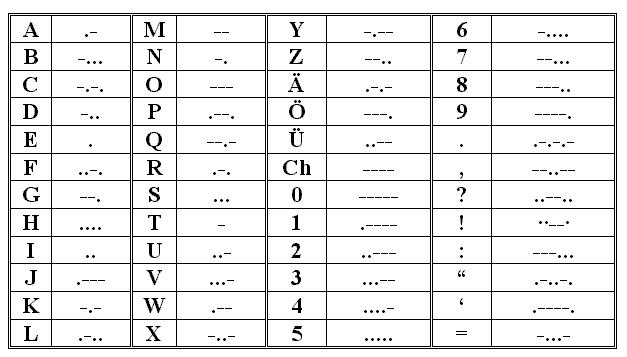
\includegraphics[scale=0.5]{morsecode}
  \label{fig:CodigoMorse}
\end{figure}


\end{frame} 

%%%%%%%%%%%%%%%%%%%%%%%%%%%%%%%%%
\subsection{Código ASCII}
\begin{frame} \frametitle{Código ASCII}

\begin{figure}
  \centering
    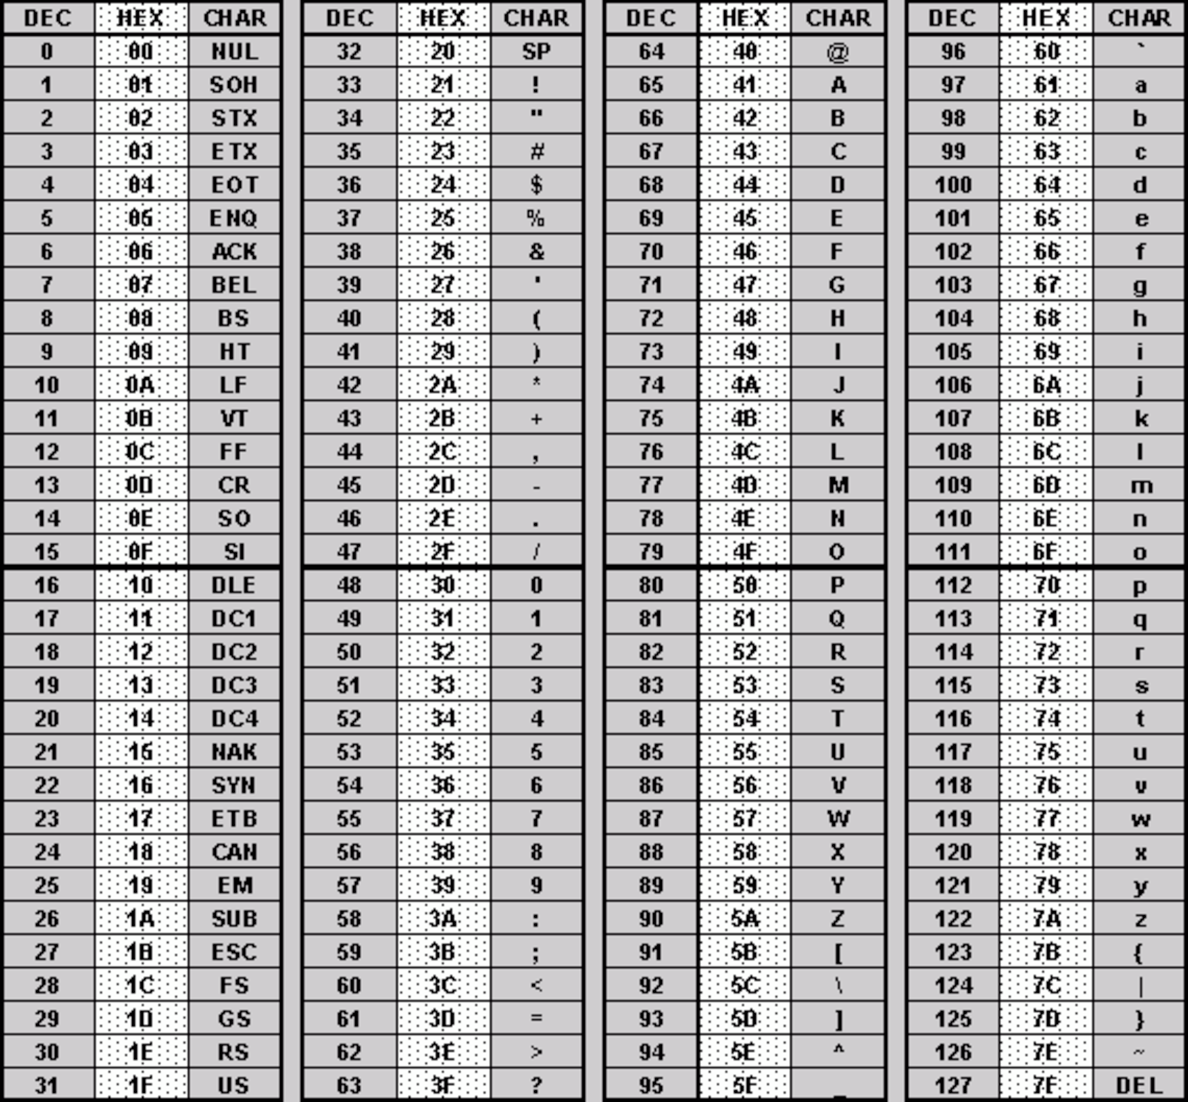
\includegraphics[scale=0.35]{ASCII}
 \label{fig:ASCII}
\end{figure}

%%%%%%%%%%%%%%%%%%%%%%%%%%%%%%%%%

\end{frame} 
\subsection{Codificación PEM}
\begin{frame} \frametitle{Codificación PEM}

 \begin{figure}[!hbtp]
\begin{minipage}{0.45\textwidth}
\begin{center}
	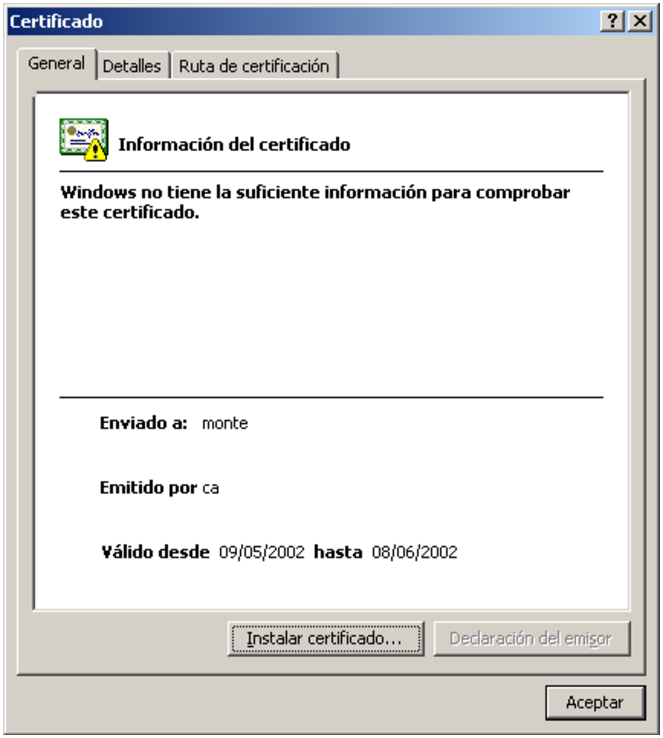
\includegraphics[scale=0.4]{Certificado} 
		  \caption{Certificado Clave Pública. Windows}
\end{center}
\end{minipage}
\hfill
\begin{minipage}{0.45\textwidth}
\begin{center}
	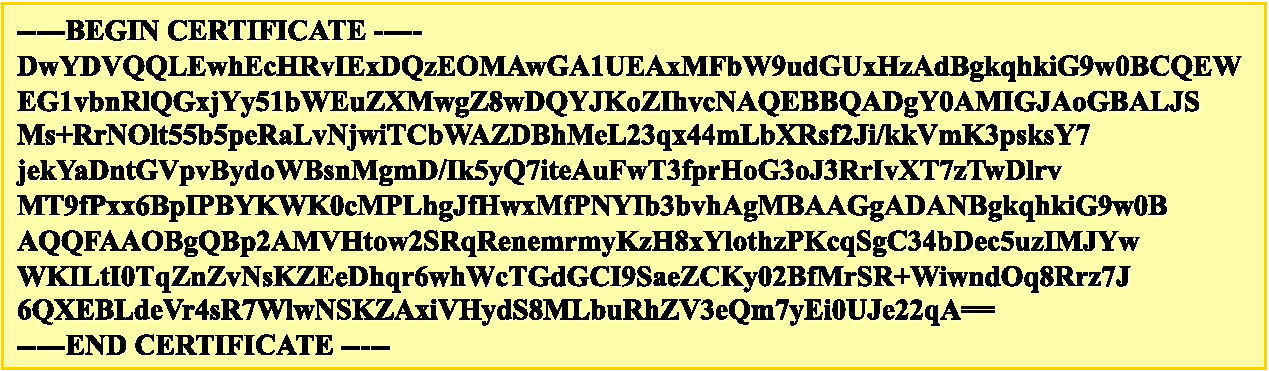
\includegraphics[scale=0.25]{PEM} 
	  \caption{Certificado Clave Pública. PEM}
\end{center}
\end{minipage}

\end{figure}

\end{frame} 

%%%%%%%%%%%%%%%%%%%%%%%%%%%%%%%%%

\subsection{Codificación de datos 2D}

\begin{frame} \frametitle{Codificación de datos 2D}

 \begin{figure}[!hbtp]
\begin{minipage}{0.45\textwidth}
\begin{center}
	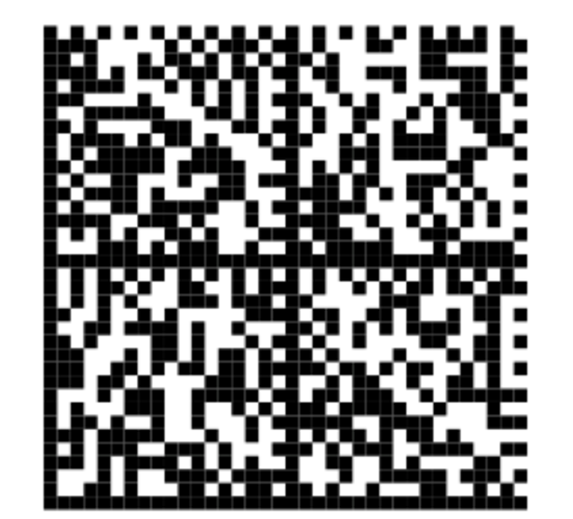
\includegraphics[scale=0.45]{Datamatrix} 
		  \caption{Datamatrix}
\end{center}
\end{minipage}
\hfill
\begin{minipage}{0.45\textwidth}
\begin{center}
	
\includegraphics[scale=0.18]{QRCode} 
	  \caption{QRCode}
\end{center}
\end{minipage}

\end{figure}

\end{frame} 


%%%%%%%%%%%%%%%%%%%%%%%%%%%%%%%%%
\subsection{Ejemplo Doble Codificación}

\begin{frame} \frametitle{Ejemplo Doble Codificación}


 \begin{figure}[!hbtp]
\begin{center}
	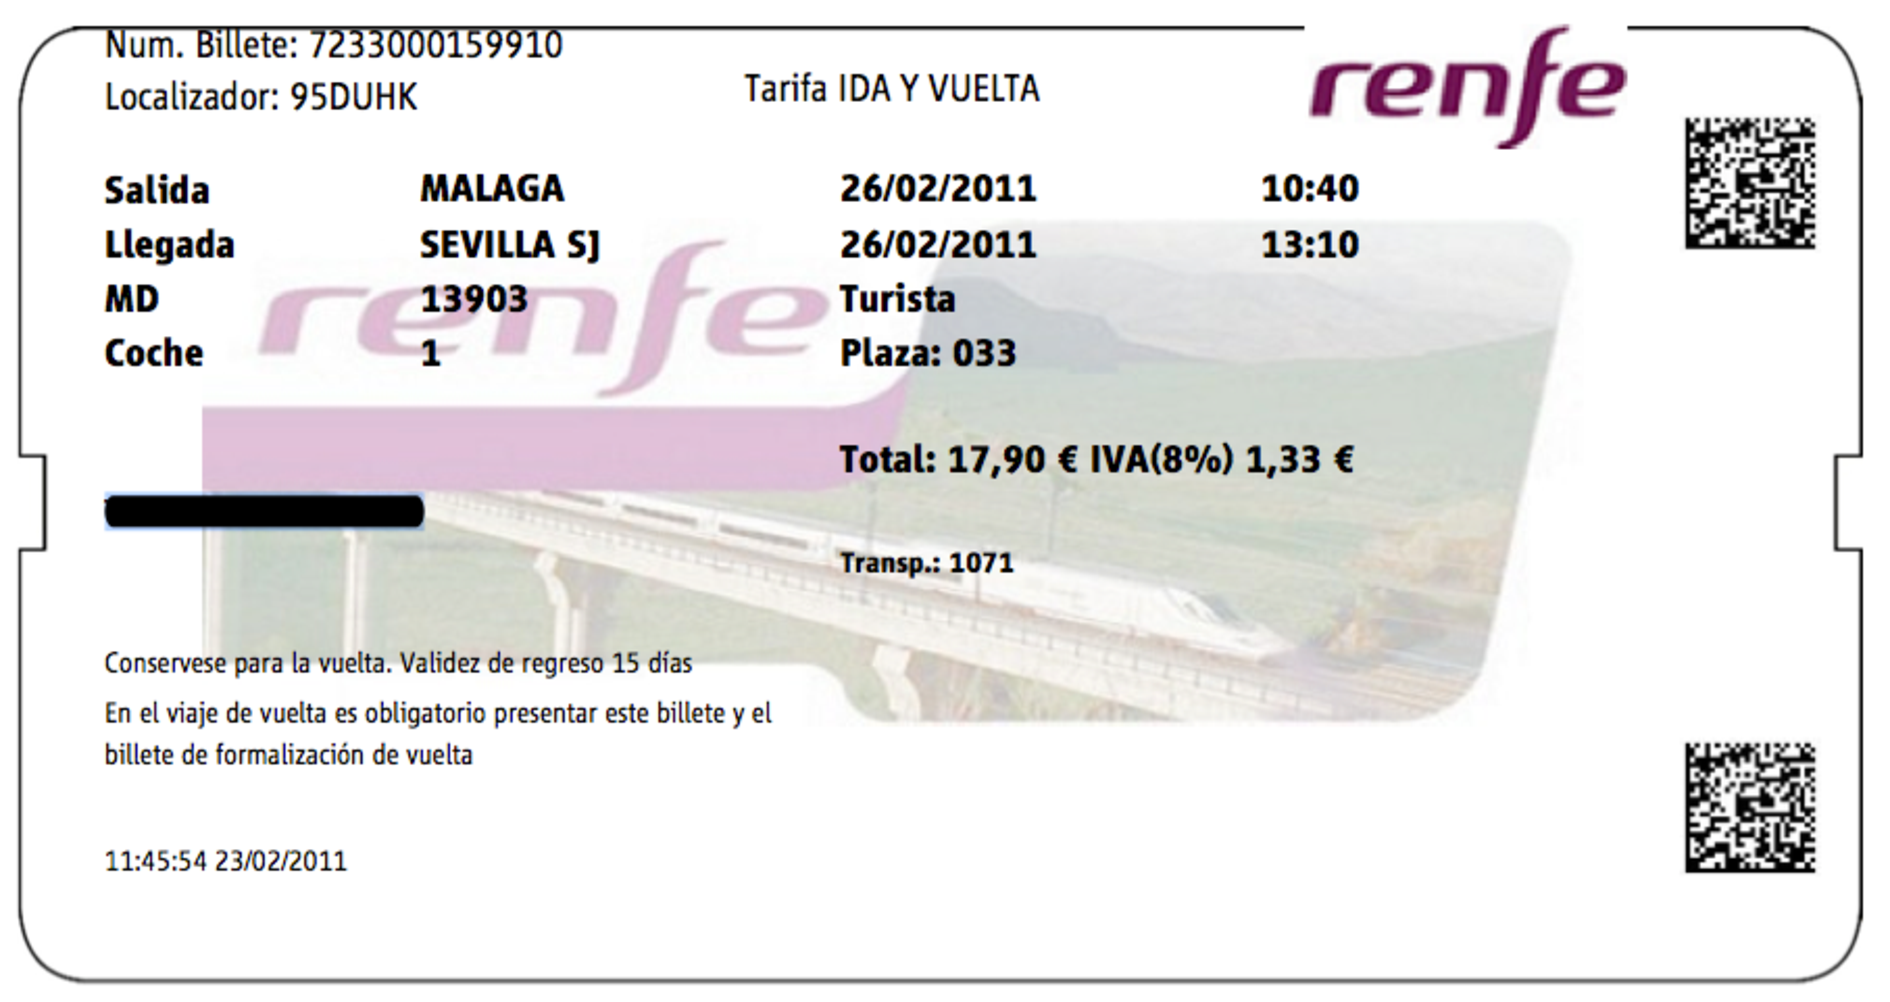
\includegraphics[scale=0.25]{RenfeIDA} 
		  \caption{Billete de IDA}
\end{center}
\end{figure}

723300015991054413510032602111390300103301695DUHK

\end{frame} 


%%%%%%%%%%%%%%%%%%%%%%%%%%%%%%%%%
\begin{frame} 


 \begin{figure}[!hbtp]
\begin{center}
	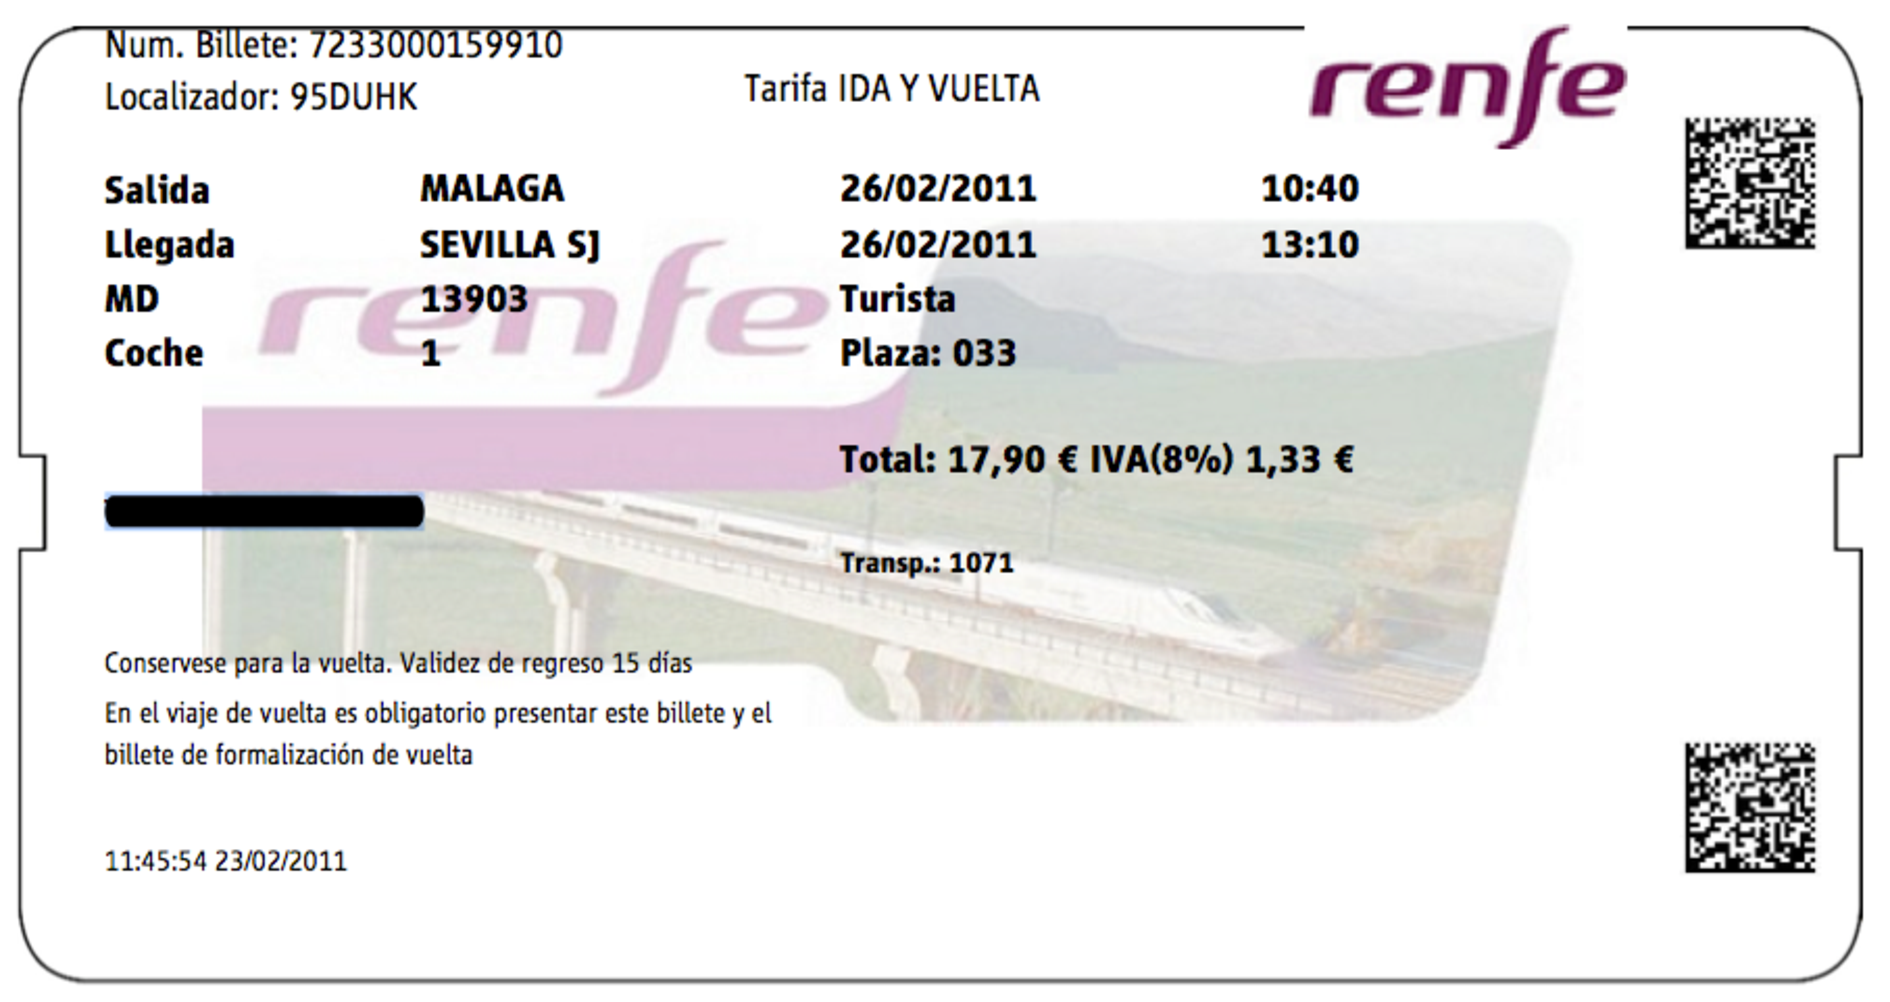
\includegraphics[scale=0.15]{RenfeIDA} 
\end{center}
\end{figure}

\small
\textbf{7233000159910}  5441351003 \textbf{260211} \textbf{13903} \textbf{001} \textbf{033} 016   \textbf{95DUHK}


\begin{description}
\item[Num. Billete:] 7233000159910

\item[Fecha:] 260211
\item[MD:] 13903
\item[Coche:] 001
\item[Plaza:] 033
\item[Localizador:] 95DUHK
\end{description}


\end{frame} 

\begin{frame} 


 \begin{figure}[!hbtp]
\begin{center}
	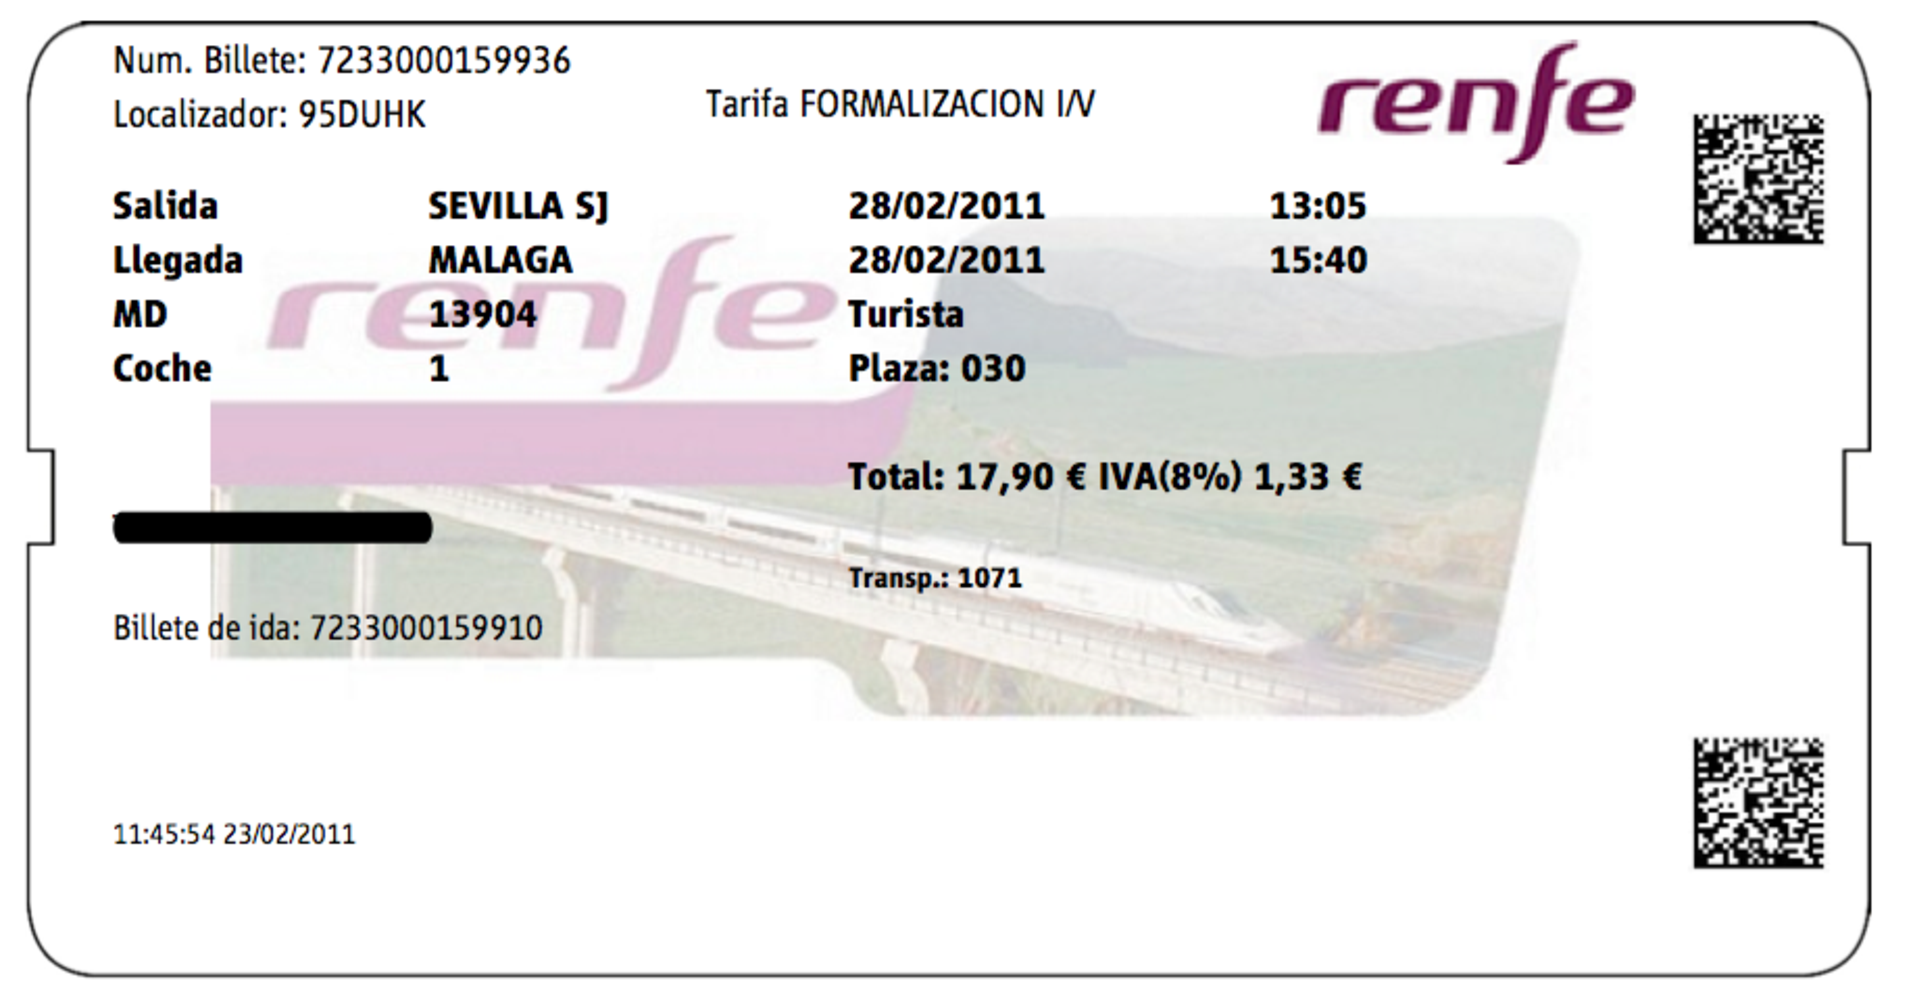
\includegraphics[scale=0.25]{RenfeVuelta} 
		  \caption{Billete de Vuelta}
\end{center}
\end{figure}

\small

\textbf{7233000159910}  5441351003 \textbf{260211} \textbf{13903} \textbf{001} \textbf{033} 016   \textbf{95DUHK}

\textbf{7233000159936}  5100354413  \textbf{280211} \textbf{13904} \textbf{001} \textbf{030} 018   \textbf{95DUHK}
                                   

\end{frame} 


\begin{frame} %\frametitle{Preguntas}

%\begin{center}
%¡Gracias por su atención!\\
%\end{center}
\vspace*{2cm}

\begin{center}
\textbf{José A. Montenegro Montes} \\

\textit{Dpto. Lenguajes y Ciencias de la Computación}\\
\textit{ETSI  Informática. Universidad de Málaga}\\
\textbf{jmmontes@uma.es}\\
%\href{https://twitter.com//monteDocencia}{
%
\includegraphics[height=0.05\textheight]{twitter.jpg}}
\end{center}

\vspace*{1,5cm}


\includegraphics[height=0.15\textheight]{logoUma.jpg} \hspace*{3.6cm}

\includegraphics[height=0.15\textheight]{logoInf.jpg}   \hspace*{3.7cm}

\includegraphics[height=0.15\textheight]{logoLcc.jpg}  




\end{frame} 

\end{document} 